%
% This is the LaTeX template file for lecture notes for EE 382C/EE 361C.
%
% To familiarize yourself with this template, the body contains
% some examples of its use.  Look them over.  Then you can
% run LaTeX on this file.  After you have LaTeXed this file then
% you can look over the result either by printing it out with
% dvips or using xdvi.
%
% This template is based on the template for Prof. Sinclair's CS 270.

\documentclass[twoside]{article}
\setlength{\oddsidemargin}{0.25 in}
\setlength{\evensidemargin}{-0.25 in}
\setlength{\topmargin}{-0.6 in}
\setlength{\textwidth}{6.5 in}
\setlength{\textheight}{8.5 in}
\setlength{\headsep}{0.75 in}
\setlength{\parindent}{0 in}
\setlength{\parskip}{0.1 in}
\usepackage{graphics}
\usepackage{amsmath}
\usepackage{tikz}
\usepackage{textcomp}
\usepackage{semantic}
\usepackage{cancel}
\usetikzlibrary{decorations.markings}
\usetikzlibrary{positioning, shapes, arrows}

%
% The following commands set up the lecnum (lecture number)
% counter and make various numbering schemes work relative
% to the lecture number.
%
\newcounter{lecnum}
\renewcommand{\thepage}{\thelecnum-\arabic{page}}
\renewcommand{\thesection}{\thelecnum.\arabic{section}}
\renewcommand{\theequation}{\thelecnum.\arabic{equation}}
\renewcommand{\thefigure}{\thelecnum.\arabic{figure}}
\renewcommand{\thetable}{\thelecnum.\arabic{table}}

%
% The following macro is used to generate the header.
%
\newcommand{\lecture}[4]{
   \pagestyle{myheadings}
   \thispagestyle{plain}
   \newpage
   \setcounter{lecnum}{#1}
   \setcounter{page}{1}
   \noindent
   \begin{center}
   \framebox{
      \vbox{\vspace{2mm}
    \hbox to 6.28in { {\bf EE 382N: Distributed Systems
                        \hfill Fall 2017} }
       \vspace{4mm}
       \hbox to 6.28in { {\Large \hfill Lecture #1: #2  \hfill} }
       \vspace{2mm}
       \hbox to 6.28in { {\it Lecturer: #3 \hfill Scribe: #4} }
      \vspace{2mm}}
   }
   \end{center}
   \markboth{Lecture #1: #2}{Lecture #1: #2}
   %{\bf Disclaimer}: {\it These notes have not been subjected to the
   %usual scrutiny reserved for formal publications.  They may be distributed
   %outside this class only with the permission of the Instructor.}
   \vspace*{4mm}
}

%
% Convention for citations is authors' initials followed by the year.
% For example, to cite a paper by Leighton and Maggs you would type
% \cite{LM89}, and to cite a paper by Strassen you would type \cite{S69}.
% (To avoid bibliography problems, for now we redefine the \cite command.)
% Also commands that create a suitable format for the reference list.
\renewcommand{\cite}[1]{[#1]}
\def\beginrefs{\begin{list}%
        {[\arabic{equation}]}{\usecounter{equation}
         \setlength{\leftmargin}{2.0truecm}\setlength{\labelsep}{0.4truecm}%
         \setlength{\labelwidth}{1.6truecm}}}
\def\endrefs{\end{list}}
\def\bibentry#1{\item[\hbox{[#1]}]}

%Use this command for a figure; it puts a figure in wherever you want it.
%usage: \fig{NUMBER}{SPACE-IN-INCHES}{CAPTION}
\newcommand{\fig}[3]{
			\vspace{#2}
			\begin{center}
			Figure \thelecnum.#1:~#3
			\end{center}
	}

\newcommand{\mymk}[1]{%
  \tikz[baseline=(char.base)]\node[anchor=south west, draw,rectangle, rounded corners, inner sep=2pt, minimum size=7mm,
    text height=2mm](char){\ensuremath{#1}} ;}


% Use these for theorems, lemmas, proofs, etc.
\newtheorem{theorem}{Theorem}[lecnum]
\newtheorem{lemma}[theorem]{Lemma}
\newtheorem{proposition}[theorem]{Proposition}
\newtheorem{claim}[theorem]{Claim}
\newtheorem{corollary}[theorem]{Corollary}
\newtheorem{definition}[theorem]{Definition}
\newenvironment{proof}{{\bf Proof:}}{\hfill\rule{2mm}{2mm}}

% **** IF YOU WANT TO DEFINE ADDITIONAL MACROS FOR YOURSELF, PUT THEM HERE:

\begin{document}
%FILL IN THE RIGHT INFO.
%\lecture{**LECTURE-NUMBER**}{**DATE**}{**LECTURER**}{**SCRIBE**}
\lecture{1}{August 31}{Vijay Garg}{Asad Malik}
%\footnotetext{These notes are partially based on those of Nigel Mansell.}

% **** YOUR NOTES GO HERE:

% Some general latex examples and examples making use of the
% macros follow.  
%**** IN GENERAL, BE BRIEF. LONG SCRIBE NOTES, NO MATTER HOW WELL WRITTEN,
%**** ARE NEVER READ BY ANYBODY.
\section*{Introduction}
Students in EE 382N are required to scribe lecture notes for one lecture.
These lecture notes will be done using the document processing system called Latex.
There is a sample {\em scribe.tex} file on the Canvas system which can be used as a template. You can run {\tt pdflatex}
on that file to generate {\em scribe.pdf}.

During each class, the professor will list the topics to be covered on the whiteboard.
Once a topic has been completed, he will check it off the list. That's the time to ask questions.

\textbf {Textbook}: Elements of Distributed Computing

The textbook will cover roughly 50\% of the course material. The rest will be covered by lectures and research papers.
There will be 3 tests during the semester and \textbf {no} final exam. Test dates will be posted on canvas.

\subsection*{Course Rules}
\begin{itemize}
  \item No cellphone or laptop use allowed during the lecture
  \item Tablets are permitted for the sole purpose of taking lecture notes
  \item Ask at least one question during the semester
  \item Limit yourself to 5 questions during a lecture
  \item No guns allowed in the office
\end{itemize}

\subsection*{Course Info}
\begin{itemize}
  \item Prof. Garg Office: EER 7.884
  \item TA: Changyong Hu (colinhu9@gmail.com)
  \item Assignments done in groups of 2
  \item Term project done in teams of 3-4
\end{itemize}

\section*{Goals of the Course}

\begin{center}
\begin{tikzpicture}
\node (A) [cloud, draw,cloud puffs=10,cloud puff arc=120, aspect=2, inner ysep=1em] {Distributed Systems};
\node (B)[draw,shape=rounded rectangle,  below left=of A,
minimum width=1.8cm]  {Algorithms};
\node (C)[draw,shape=rounded rectangle,  below right=of A,
minimum width=1.8cm]  {Systems};
\draw [->] (A) edge (B) (A) edge (C);
\end{tikzpicture}
\end{center}

Both \textbf{Algorithms} and \textbf{Systems} are an important part of this course. We will be covering the theory as well as putting it into practice
so expect to work on complex programming assigments.

The term project is a very important part of the course. The goal is to produce something new instead of working on already solved problems.
The term project is loosely based on a conference style of submission with each team submitting a paper (7-8 pages) which will be reviewed by their peers. 
Papers which are accepted by the reviewers will be presented at the end of the semester. The deadline for submission will be 2-3 weeks prior to the end of
the semester (exact dates are TBD). You will be expected to study and work in groups as collaboration is a good way to learn the material.

\section*{Happened-before, Posets \& Lattices}

\textbf {Source}: Lamport's paper '78 \textit Time, Clocks, and the Ordering of Events in a Distributed System


\textbf {Definition} of Distributed Systems. 
There are 3 assumptions associated with what a distributed system is:
\begin{enumerate}
  \item No shared clocks
  \item No shared memory
  \item Asynchronous
\end{enumerate}

\begin{center}
\begin{tikzpicture}
\node (A) [cloud, draw,cloud puffs=10,cloud puff arc=120, aspect=2, inner ysep=1em] {Network};
\node (B)[draw,shape=rounded rectangle,  below left=of A,
minimum width=1.8cm]  {P1};
\node (C)[draw,shape=rounded rectangle,  below right=of A,
minimum width=1.8cm]  {P2};
\draw [-] (A) edge (B) (A) edge (C);
\end{tikzpicture}
\dots
\end{center}

The only way for communication is through messages which may take an unbounded amount of time.
There is no way to synchronize the clocks due to uncertainity of how long messages might take.

Lamport's paper discusses how to order events with asynchronous clocks.

Defining happened-before \textbf{(\textrightarrow)} without using clocks:

If we say e \textbf{\textrightarrow} f, we much be 100\% certain of the fact.
Rules for \textbf{\textrightarrow} relations.  \textbf{\textrightarrow} is the smallest relation such that:
\begin{itemize}
	\item if e occured before f in the same process, then e \textbf{\textrightarrow} f
	\item if e is send of a message and f is the receive of that message, then e  \textbf{\textrightarrow} f
	\item if $\exists$ g: e  \textbf{\textrightarrow} g $\land$ g  \textbf{\textrightarrow} f, then e  \textbf{\textrightarrow} f
\end{itemize}

\textbf{Example:}

\tikzset{->-/.style={decoration={
  markings,
  mark=at position #1 with {\arrow{>}}},postaction={decorate}}}

\begin{tikzpicture}
% a straight line segment
\draw[-latex] (-2,0) -- (2,0);
% the ticks and their labels
 \draw[xshift=-1.75 cm] (0pt,2pt) -- (0pt,-1pt) node[below,fill=white] (e1) {e1};
 \draw[xshift= 0 cm] (0pt,2pt) -- (0pt,-1pt) node[below,fill=white] (e2) {e2};
 \draw[xshift=1.5 cm] (0pt,2pt) -- (0pt,-1pt) node[below,fill=white] (e3) {e3};


% a straight line segment
\draw[-latex] (-2,-2) -- (2,-2);
% the ticks and their labels
 \draw[xshift=-1.75 cm, yshift=-2 cm] (0pt,2pt) -- (0pt,-1pt) node[below,fill=white] (f1) {f1};
 \draw[xshift= 0 cm, yshift=-2 cm] (0pt,2pt) -- (0pt,-1pt) node[below,fill=white] (f2) {f2};
 \draw[xshift=1.5 cm, yshift=-2 cm] (0pt,2pt) -- (0pt,-1pt) node[below,fill=white] (f3) {f3};

\draw [blue, solid, ->] (0,0) -- (1.5,-2);
\end{tikzpicture}

From the example, we can infer the following:
\begin{enumerate}
  \item  e1 \textbf{\textrightarrow} e2,  e2 \textbf{\textrightarrow} e3, hence  e1 \textbf{\textrightarrow} e3
  \item  f1 \textbf{\textrightarrow} f2, f2 \textbf{\textrightarrow} f3, hence f1 \textbf{\textrightarrow} f3
  \item  e2 \textbf{\textrightarrow} f3 (message sent at e2 received at f3) hence e1 \textbf{\textrightarrow} f3
\end{enumerate}

\textbf{Concurrent Events:} e $||$ f $ \implies $ (e  \cancel{\textrightarrow} f) $\land$ (f \cancel{\textrightarrow} e)

\textrightarrow is transitive. \\
\textrightarrow is irreflexive; no event can happen before itself just like $<$ "less than" relationship. \\
\textrightarrow defines relationships in the irreflexive partially ordered set.

Examples of \textbf{irreflexive asymmetric}
\begin{itemize}
	\item (E, \textrightarrow)
	\item (N, $<$)
\end{itemize}
where: \\
E is the set of all relationships defined by \textrightarrow relationship \\
N is the set of all natural numbers defined by $<$ relationship


Examples of \textbf{reflexive antisymmetric}
\begin{itemize}
	\item (E, \underline{\textrightarrow})
	\item (N, $\leq$)
\end{itemize}
where: \\
E is the set of all relationships defined by \underline{\textrightarrow}relationship \\
N is the set of all natural numbers defined by $\leq$ relationship

(e  \underline{\textrightarrow} f) $\land$ (f  \underline{\textrightarrow} e) $\implies$ e = f


\subsection*{Posets}

\underline {Hasse Diagram} transitively reduced diagram 


\begin{tikzpicture}[scale=.7]
  \node (c) at (-2,2) {$c$};
  \node (e) at (2,2) {$e$};
  \node (b) at (-2,0) {$b$};
  \node (d) at (2,0) {$d$};
  \node (a) at (0,-2) {$a$};
  \draw (a) -- (b) -- (c) -- (b) -- (a) -- (d) -- (e) -- (d);
\end{tikzpicture}

a $<$ b, a $<$ c \\
a $<$ d, a $<$ e \\
b $<$ c, d $<$ e \\
 
\textbf{Chain:} Y is a chain in X if \\ $\forall$ a,b $\in$ Y: (a $\leq$ b) $\lor$ (b $\leq$ a) \\
\textbf{Example:} Longest chains are (a,b,c) and (a,d,e). [Length is 3] \\

\textbf{Anti-Chain:} Y is an anti-chain in X if \\ $\forall$ a,b $\in$ Y: (a $||$ b) \\
\textbf{Example:} Longest anti-chains are (b,d), (c,e), (c,d), (b,d). [Width is 2]

\textbf{Note:}
\begin{enumerate}
\item Height of poset is the longest chain
\item Width of poset is longest anti-chain
\end{enumerate}



\begin{center}
\textbf{Some More Examples}
\end{center} 
Relation (N, divides). a $\leq$ b if a divides b, i.e b \% a = 0

\begin{tikzpicture}[scale=.7]
  \node (six) at (0,2) {$6$};
  \node (five) at (4,0) {$5$};
  \node (four) at (-2,2) {$4$};
  \node (three) at (2,0) {$3$};
  \node (two) at (-2,0) {$2$};
  \node (one) at (0,-2) {$1$};
  \draw (one) -- (two) -- (four);
  \draw (one) -- (five);
  \draw (one) -- (three) -- (six);
  \draw (two) -- (six);
\end{tikzpicture}


Set Y = {a, b}
Subsets of Y:
\begin{tikzpicture}[scale=.7]
  \node (ab) at (0,2) {$\{a, b\}$};
  \node (empty) at (0,-2) {$\{\}$};
  \node (b) at (2,0) {$\{b\}$};
  \node (a) at (-2,0) {$\{a\}$};
  \draw (empty) -- (a) -- (ab);
  \draw (empty) -- (b) -- (ab);
\end{tikzpicture}


\subsection*{Infimum and Supremum}

\textbf{Infimum} \\ 
Given (X, $\leq$) \& Y $\subseteq$ X

m $\in$ X is the meet/infimum/"greatest lower bound" of Y if
\begin{enumerate}
	\item $\forall$ y $\in$ Y: m $\leq$ y \{m is a lower bound\}
	\item $\forall$ m' : [$\forall$ y $\in$ Y: m' $\leq$ y] $\implies$ m' $\leq$ m
\end{enumerate}



\begin{tikzpicture}[scale=.7]
  \node (c) at (-2,2) {$c$};
  \node (e) at (2,2) {$e$};
  \node (b) at (-2,0) {$b$};
  \node (d) at (2,0) {$d$};
  \node (a) at (0,-2) {$a$};
 \node (q) at (0,-3.5) {$q$};
 \node (r) at (0,-5) {$r$};
  \draw (r) -- (q) -- (a) -- (b) -- (c) -- (b) -- (a) -- (d) -- (e) -- (d);
\end{tikzpicture}

\textbf {inf} (b,e) = a = b  \textbf{$\sqcap$} e \\
\textbf {inf} is represented by the symbol ($\sqcap$)

\textbf{Supremum} \\
Supremum is the least upper bound and is represented by the symbol (\textbf{$\sqcup$}). For the example above, the sup(b,e) or b $\sqcup$ e does not exist.

A poset (X, $\leq$) is a lattice if for all \underline{finite} Y $\subseteq$ X, sup(Y) and inf(Y) exist.


\begin{tikzpicture}[scale=.7]
  \node (f) at (0, 4) {$f$};
  \node (c) at (-2,2) {$c$};
  \node (e) at (2,2) {$e$};
  \node (b) at (-2,0) {$b$};
  \node (d) at (2,0) {$d$};
  \node (a) at (0,-2) {$a$};
 \node (q) at (0,-3.5) {$q$};
 \node (r) at (0,-5) {$r$};
  \draw (r) -- (q) -- (a) -- (b) -- (c) -- (b) -- (a) -- (d) -- (e) -- (d);
  \draw (c) -- (f) -- (e);
\end{tikzpicture}

The example above is a lattice as for all subsets, \textbf{sup} and \textbf{inf} exist. \\
b $\sqcup$ e = f \\
b $\sqcap$ e = a


\begin{tikzpicture}[scale=.7]
  \node (f) at (0, 4) {$f$};
  \node (d) at (-2,2) {$d$};
  \node (e) at (2,2) {$e$};
  \node (b) at (-2,0) {$b$};
  \node (c) at (2,0) {$c$};
  \node (a) at (0,-2) {$a$};
  \draw (a) -- (b) -- (d) -- (f) -- (e) -- (c) -- (a);
 \draw (b) -- (e);
  \draw (c) -- (d);
\end{tikzpicture}

The example above is \textbf{NOT} a lattice. \\
b $\sqcup$ c = does not exist \\
b $\sqcap$ c = a

For (N, divides) poset, GCD = inf and LCM = sup.


\textbf {Distributive Property}:
\begin{enumerate}
\item a  $\sqcap$ ( b $\sqcup$ c) = (a $\sqcap$ b) $\sqcup$ (a $\sqcap$ c) 
\item a  $\sqcup$ ( b $\sqcap$ c) = (a $\sqcup$ b) $\sqcap$ (a $\sqcup$ c) 
\end{enumerate}


\textbf {Pentagon Lattice}

\begin{tikzpicture}[scale=.7]
  \node (f) at (0, 4) {$f$};
  \node (d) at (-2,2) {$d$};
  \node (e) at (2,2) {$e$};
  \node (c) at (2,0) {$c$};
  \node (a) at (0,-2) {$a$};
  \draw (a) -- (d) -- (f) -- (e) -- (c) -- (a);
\end{tikzpicture}


The lattice above is not distributive.

\textbf {Diamond Lattice}

\begin{tikzpicture}[scale=.7]
  \node (e) at (0, 4) {$e$};
  \node (d) at (2,2) {$d$};
  \node (b) at (-2,2) {$b$};
  \node (c) at (0,2) {$c$};
  \node (a) at (0,-2) {$a$};
  \draw (a) -- (d) -- (e) -- (c) -- (a) -- (b) -- (e);
\end{tikzpicture}



\end{document}





